\begin{frame}{Biological Analogy}
	\begin{figure}[H]
		\centering
		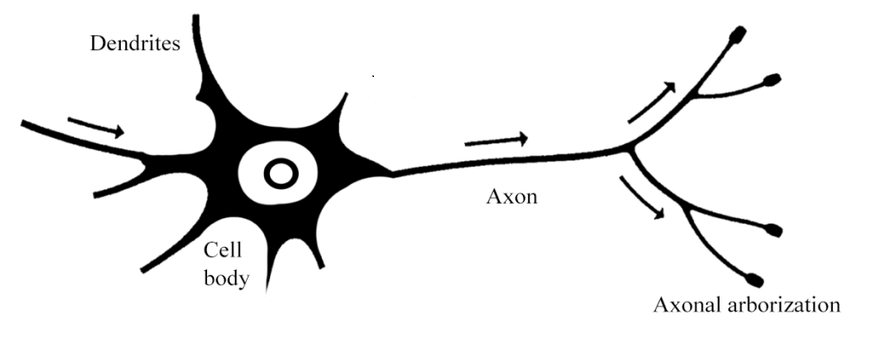
\includegraphics[width=0.9\textwidth]{Figs/biological_neuron.png}
		\caption{Anatomy of a biological neuron \cite{biological-and-nn-neuron}.}
	\end{figure}
\end{frame}

\begin{frame}{Activation Functions}
	\begin{figure}[H]
		\centering
		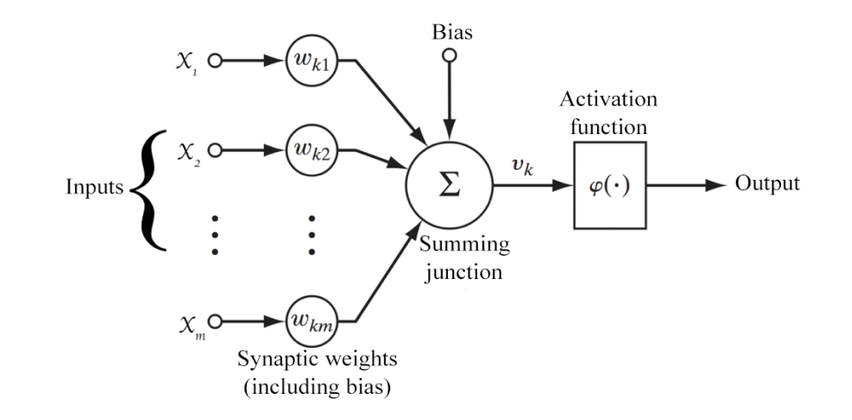
\includegraphics[width=0.9\textwidth]{Figs/nn_neuron.png}
		\caption{Neural network neuron \cite{biological-and-nn-neuron}.}
	\end{figure}
\end{frame}

\begin{frame}{Activation Functions}
	\begin{figure}[H]
		\centering
		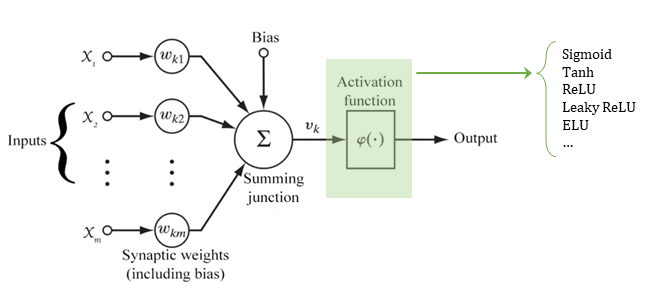
\includegraphics[width=0.9\textwidth]{Figs/activation_function_1.png}
		\caption{Activation function}
	\end{figure}
\end{frame}

\begin{frame}{Activation Functions}
	\begin{figure}[H]
		\centering
		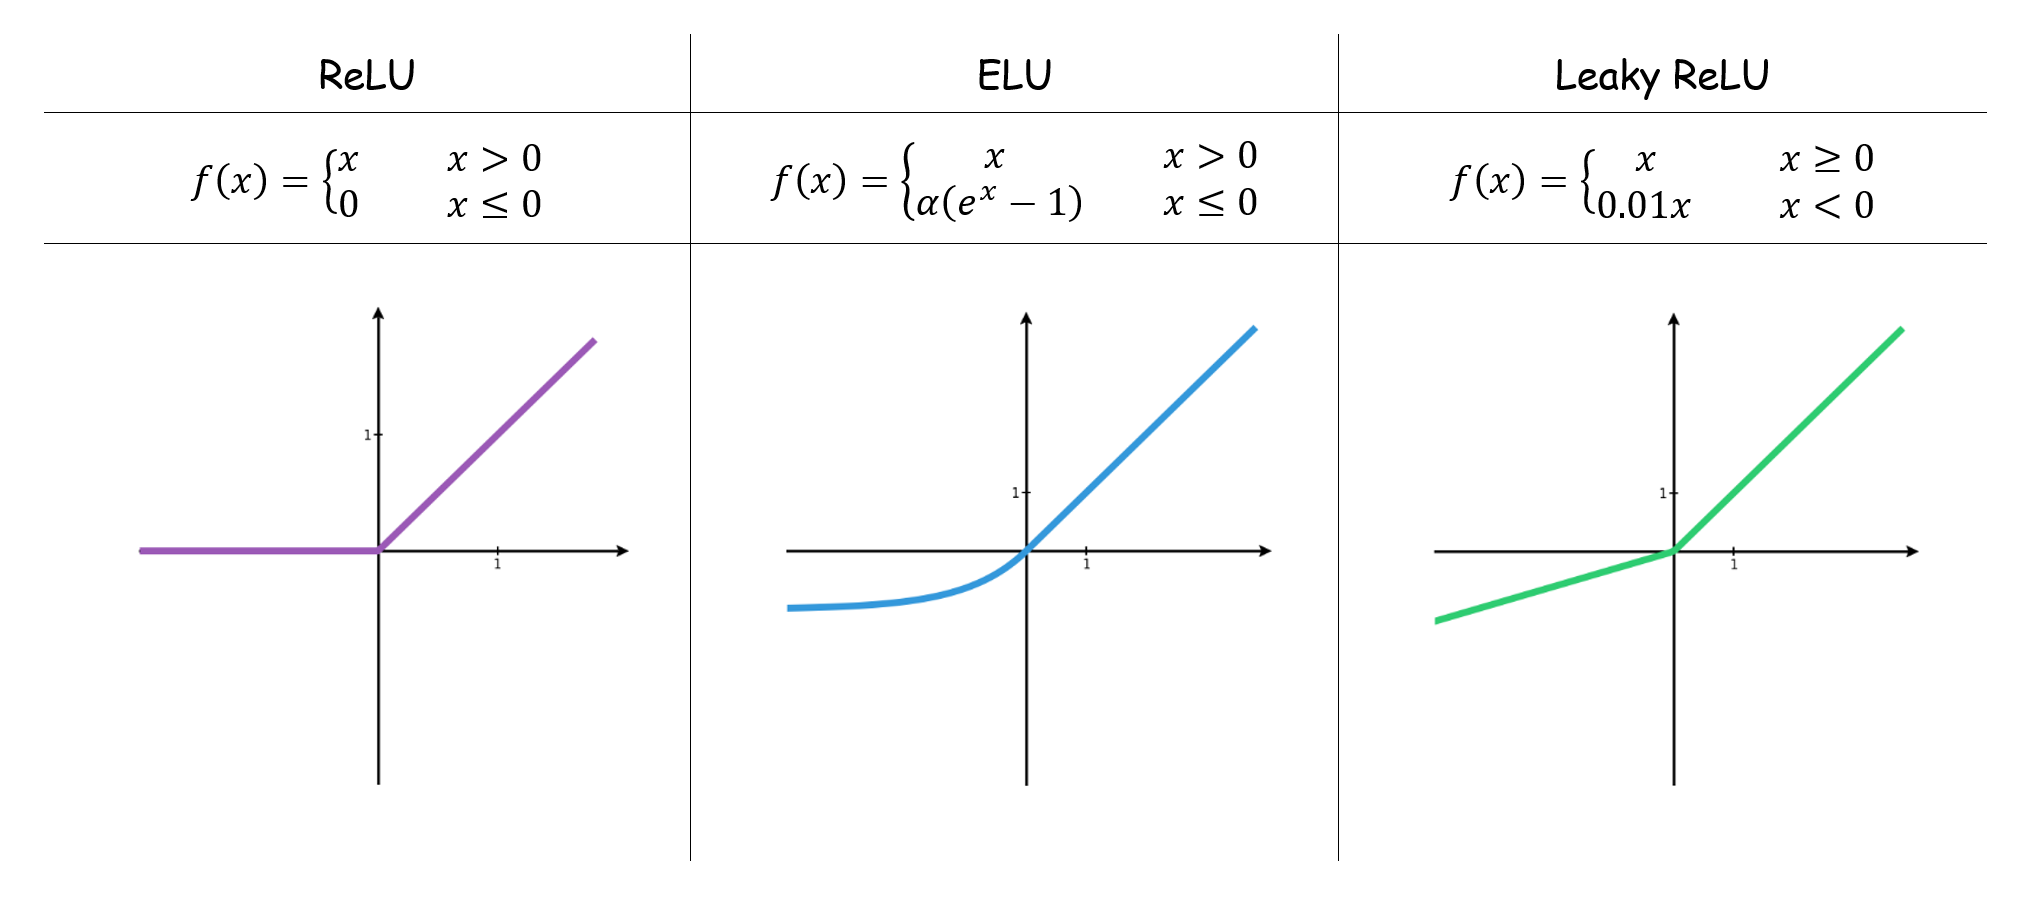
\includegraphics[width=1\textwidth]{Figs/section_1/activation_functions_1.PNG}
	\end{figure}
\end{frame}

\begin{frame}{Activation Functions}
	\begin{figure}[H]
		\centering
		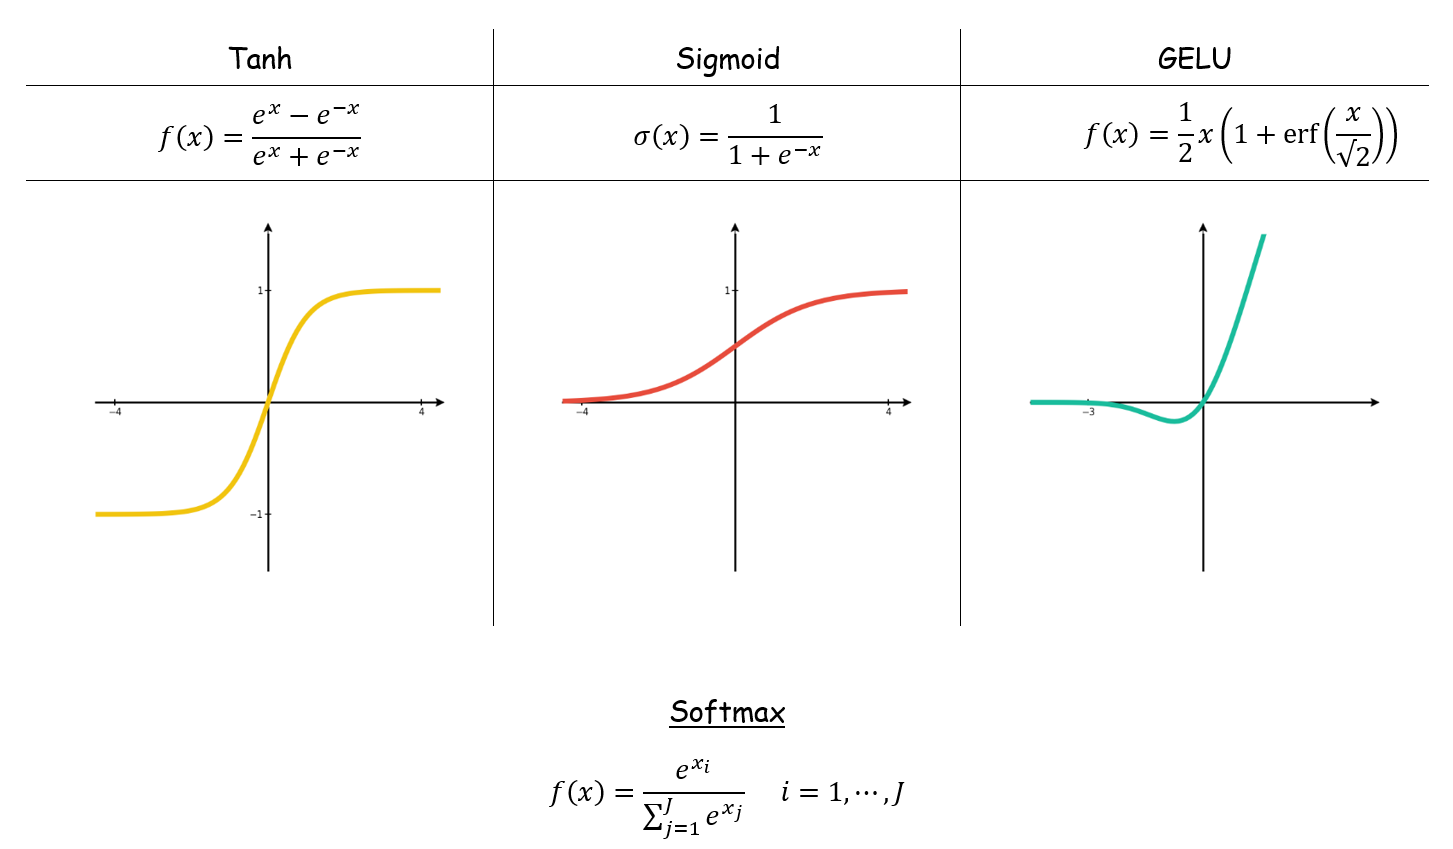
\includegraphics[width=1\textwidth]{Figs/section_1/activation_functions_2.PNG}
	\end{figure}
\end{frame}

\begin{frame}{Gradient Descent}
	\begin{figure}[H]
		\centering
		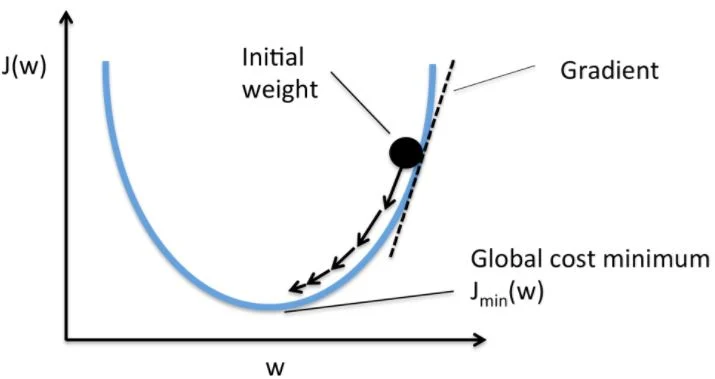
\includegraphics[width=0.70\textwidth]{Figs/gradient_descent2.png}
		\caption{Gradient descent \cite{gradient-descend2}.}
	\end{figure}
\end{frame}

\begin{frame}{Gradient Descent}
	\begin{itemize}
		\item Let's define our problem:
		\begin{itemize}
			\item We have dataset $\mathcal{D} = \{x^{i}, y^{(i)}\}_{i=1}^{n}$.
			\medskip
			\item $f$ is a single layer perceptron.
			\medskip
			\item Define $\hat{y}^{(i)} = f(x^{(i)})$.
		\end{itemize}
		\medskip
		\item We want to minimize following cost function:
		$$
		\mathcal{J}(\bm{w})  = \frac{1}{2} \sum_{i=1}^{n} (y^{(i)} - \hat{y}^{(i)})^2
		$$
		\medskip
		\item We are going to use gradient descent algorithm. $\bm{w}$ will be updated as follows:
		\[
		\bm{w}^{t+1} = \bm{w}^{t} - \eta \nabla_{\bm{w}} \mathcal{J}
		\]
	\end{itemize}
\end{frame}

\begin{frame}{Gradient Descent}
	\begin{itemize}
		\item Let's find $\nabla_{\bm{w}} \mathcal{J}$:
	\end{itemize}
	\vspace*{0.5em}
	\begin{equation*} 
		\begin{split}
			\frac{\partial J}{\partial w_j} & = \frac{\partial }{\partial w_j} \frac{1}{2} \sum_i  (y^{(i)} - \hat{y}^{(i)})^2 \\
			& = \frac{1}{2} \sum_i \frac{\partial}{\partial w_j} (y^{(i)} - \hat{y}^{(i)})^2 \\
			& = \frac{1}{2} \sum_i 2 (y^{(i)} - \hat{y}^{(i)}) \frac{\partial}{\partial w_j} (y^{(i)} - \hat{y}^{(i)}) \\ 
			& = \sum_i (y^{(i)} - \hat{y}^{(i)}) \frac{\partial}{\partial w_j} \bigg(y^{(i)} - \sum_j w_j x^{(i)}_{j}\bigg) \\
			& = \sum_i  (y^{(i)} - \hat{y}^{(i)})(-x^{(i)}_{j}) 
		\end{split}
	\end{equation*}
	
	$$\Delta w_j = - \eta \frac{\partial J}{\partial w_j} = - \eta \sum_i  (y^{(i)} - \hat{y}^{(i)})(- x^{(i)}_{j}) = \eta \sum_i (y^{(i)} - \hat{y}^{(i)})x^{(i)}_{j}$$
	
	$$\mathbf{w} := \mathbf{w} + \Delta \mathbf{w}$$
\end{frame}